% Required packages in the main preamble:
% \usepackage{graphicx}
% \usepackage{booktabs}
% \usepackage{tabularx}
% \usepackage{array}

\providecommand{\SysName}{CARE}

\section{A Motivating Example}
\label{sec:motivating-example}

This section uses a small C function to illustrate why security-sensitive
refactoring cannot be reduced to syntactic cleanup. The function is deliberately
compact, but it contains common systems-code constraints: ownership of a pointer,
a lock-like resource, multiple error paths, different return codes, and an
externally visible side effect.

\subsection{Security-Sensitive Cleanup}
\label{sec:motivation-cleanup}

Figure~\ref{fig:motivating-code-comparison} shows the key paths in the
motivating example. The original function repeats the same cleanup sequence on
three paths: it frees
\texttt{p} when non-null, releases \texttt{lock}, and then returns a path-specific
status code. The refactored version introduces a local return variable and a
single \texttt{out} label, consolidating cleanup while preserving the original
resource-release order.

\begin{figure}[t]
  \centering
  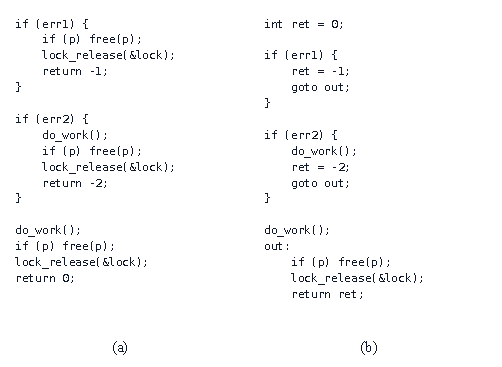
\includegraphics[width=\columnwidth]{img/care_motivating_code_comparison.pdf}
  \caption{A motivating cleanup refactoring. (a) The original code duplicates
  security-sensitive cleanup on three paths. (b) The refactored code uses one
  shared cleanup site, but it is safe only if return values, side effects, null
  checks, and lock-release behavior are preserved.}
  \label{fig:motivating-code-comparison}
\end{figure}

Although the transformation is visually small, it is guarded by path-sensitive
requirements. Table~\ref{tab:motivating-invariants} summarizes the behaviors
that any valid patch must preserve.

\begin{table}[t]
  \centering
  \caption{Safety obligations in the motivating example.}
  \label{tab:motivating-invariants}
  \footnotesize
  \begin{tabularx}{\columnwidth}{@{}>{\raggedright\arraybackslash}p{0.28\columnwidth}>{\raggedright\arraybackslash}X@{}}
    \toprule
    \textbf{Path} & \textbf{Obligation} \\
    \midrule
    \texttt{err1} &
    Return \texttt{-1}; do not call \texttt{do\_work()}; free and unlock exactly once. \\
    \texttt{err2} &
    Call \texttt{do\_work()} once; return \texttt{-2}; free and unlock exactly once. \\
    Success &
    Call \texttt{do\_work()} once; return \texttt{0}; free and unlock exactly once. \\
    Null pointer &
    Preserve the null guard before \texttt{free(p)} and avoid dereferencing \texttt{p}. \\
    \bottomrule
  \end{tabularx}
\end{table}

\subsection{LLM-Only Risk}
\label{sec:motivation-risk}

A direct LLM-only prompt can easily recognize that the cleanup is duplicated.
The hard part is not noticing repetition; it is preserving the conditions under
which each statement executes. A plausible-looking rewrite can still be unsafe
if it returns the wrong status code, moves \texttt{do\_work()} onto the
\texttt{err1} path, releases the lock before an originally protected side
effect, removes the null check before \texttt{free(p)}, or drops a cleanup action
because it appears redundant locally.

This example captures the paper's core problem. The desired edit is local, but
the safety argument is contextual: it depends on control flow, resource
lifecycle, side effects, and API-level return conventions. As a result, the
refactoring engine must reason about more than the text span being edited.

\subsection{\SysName{}'s Context-Aware Refactoring}
\label{sec:motivation-care}

\SysName{} handles the example by turning the cleanup rewrite into a constrained
patch-generation task. First, it extracts the function, builds a lightweight
context graph, and detects a cleanup-consolidation opportunity. The detector
evidence records three affected return paths and two duplicated cleanup
statements: \texttt{free(p);} and \texttt{lock\_release(\&lock);}. The context
summary records that \texttt{do\_work()} executes on the \texttt{err2} and
success paths, but not on the \texttt{err1} path.

The LLM is then asked to generate a minimal patch under explicit safety
constraints rather than to perform an unconstrained cleanup. \SysName{} validates
the candidate on a clean project tree by applying the diff, compiling the code,
running tests, and checking for resource, semantic, and security regressions. In
this example, the tests cover the \texttt{err1}, \texttt{err2}, success, and
null-pointer success paths, while the validator checks that public signatures,
return behavior, cleanup actions, and security checks are preserved.

The takeaway is that a useful LLM-based refactoring system needs three pieces to
work together: structured evidence for the opportunity, context-aware prompting
for patch generation, and conservative validation before accepting the result.
The rest of the paper describes how \SysName{} generalizes this workflow to
larger C/C++ projects.
